\documentclass{article}
\usepackage[utf8]{inputenc}

\usepackage{listings}
\usepackage{framed}
\usepackage{color}
\usepackage{graphicx}

% FOR COLORS WITH PYTHON CODE

% Default fixed font does not support bold face
\DeclareFixedFont{\ttb}{T1}{txtt}{bx}{n}{10} % for bold
\DeclareFixedFont{\ttm}{T1}{txtt}{m}{n}{10}  % for normal

% Custom colors

\definecolor{deepblue}{rgb}{0,0,0.5}
\definecolor{deepred}{rgb}{0.6,0,0}
\definecolor{deepgreen}{rgb}{0,0.5,0}

\setlength{\parindent}{0ex}

% Python style for highlighting
\newcommand\pythonstyle{\lstset{
    language=Python,
    basicstyle=\ttm,
    otherkeywords={self},             % Add keywords here
    keywordstyle=\ttb\color{deepblue},
    emph={MyClass,__init__},          % Custom highlighting
    emphstyle=\ttb\color{deepred},    % Custom highlighting style
    stringstyle=\color{deepgreen},
    frame=tb,                         % Any extra options here
    showstringspaces=false            % 
}}

% Python environment
\lstnewenvironment{python}[1][]
{
  \pythonstyle
  \lstset{#1}
}
{}

%%% END %%%

\title{Compte Rendu - Apprentissage et Reconnaissance de Formes}
\author{Michael Trazzi, Julien Denes }
\date{Mars 2018}
\pagenumbering{gobble}


\begin{document}

\maketitle


%%% BEGIN TME 1 %%%

\section*{TME 1 - Arbres de décision, sélection de modèles}

\subsection*{Calcul de l'entropie}
\begin{python}
  def entropie(vect):
  _, counts = np.unique(vect, return_counts=True)
  p_y = np.array(counts / len(vect))
  return (-np.sum(p_y * np.log(p_y)))
\end{python}

\begin{python}
  def entropie_cond(list_vect):
  n = len(list_vect)
  total_nb = sum(len(part) for part in list_vect)
  p = np.array((1,n))
  H = np.array((1, n))
  for i in range(n):
  p[i] = len(list_vect[i]) / total_nb
  H[i] = entropie(list_vect[i])
  return (np.sum(H * p))
\end{python}

\subsection*{Quelques expériences préliminaires}
\begin{figure}[h]
  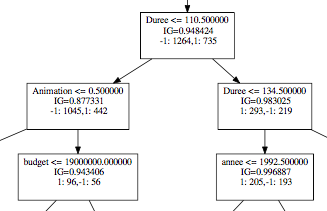
\includegraphics[width=\textwidth,
  height=\textheight,keepaspectratio]{tree5_part}
  \caption{une partie de ce qu'on obtient avec profondeur 5}
\end{figure}

\textbf{Q 1.4} Sur les données IMDB, nous avons testé des
profondeurs d'arbres allant de 5 à 50. Plus la profondeur
est grande, et plus on \underline{surapprend} notre base de
données d'apprentissage.

\textbf{Q 1.5} Pour une profondeur de 5 (resp. 50), on
obtient un score de 0.736429038587 (resp. 0.900152605189).
On a bien un \underline{surapprentissage} de nos données
dans le cas de la profondeur de 50.

\textbf{Q 1.6} Le score ainsi défini \underline{n'est pas un
indicateur fiable} : il indique uniquement notre capacité a
surapprendre la base d'apprentissage, mais ne tient pas
compte du pouvoir de généralisation.

\subsection*{Sur et sous apprentissage}

\begin{center}
  \begin{figure}
    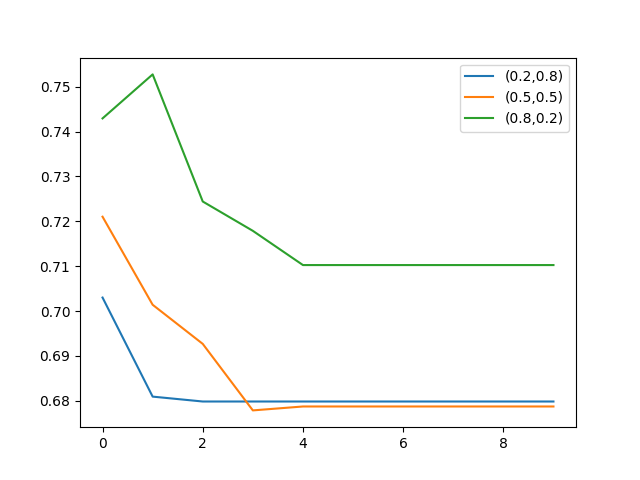
\includegraphics[width=\textwidth,
    keepaspectratio]{Figure_1}
    \caption{Evolution du score en fonction de
    (profondeur-1)/5 avec toute la base d'apprentissage}
  \end{figure}
\end{center}

\begin{center}
  \begin{figure}
    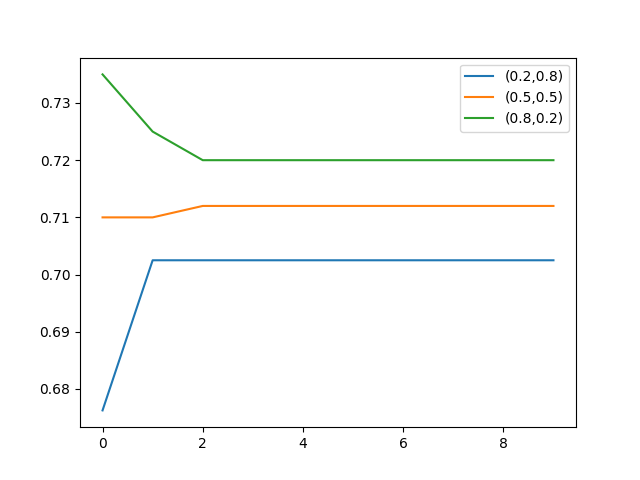
\includegraphics[width=\textwidth,
    keepaspectratio]{Figure_3}
    \caption{Idem avec peu d'exemples (1000 au lieu de
    4000)}
  \end{figure}
\end{center}


\textbf{Q 1.7} (cf. Figures 2 et 3 pour les courbes)

\textbf{Q 1.8} Avec peu d'exemples d'apprentissage, le score
se stabilise tres rapidement en fonction de la profondeur.
Avoir un arbre tres profond avec seulement 1000 exemples ne
fait pas varier le score. A contrario, avec l'ensemble de la
base d'apprentissage, le score continue a varier jusqu'a une
prondeur de 25.

\textbf{Q 1.9} Mes resultats ne me semblent pas fiables
(seulement 5 points pour chaque courbe, base d'apprentissage
de seulement quelques milliers d'exemples). Pour les
ameliorer il faudrait prendre plus d'exemples (10 000 000),
plus de répartitions (au moins 5) et plus de points (100
profondeurs différentes).


%%% END TME1 %%%





\section*{TME 2 - Estimation de densité - Expérimentations}

\subsection*{Méthode des histogrammes}

\subsection*{Méthode a noyaux}

\subsection*{Différence entre faible et forte
discrétisation}

\subsection*{Role des parametres des méthodes a noyaux}

\subsection*{Choix automatique des meilleurs parametres}

\subsection*{Estimation de la qualité du modele}

\section*{TME 3 - Descente de gradient}

\subsection*{Optimisation de fonctions}

\subsection*{Régression logistique}

\section*{TME 4 - Perceptron}

\subsection*{Implémentation}

\subsection*{Données USPS}

\subsection*{Données 2D et projection}

\end{document}
